\section{Numerical examples}

For the sake of brevity, we will focus on a more complete description of our numerical approach in our presentation.
However, it is important to understand the costs and benefits of this particular fast method, and we would like to present some characteristic examples.

As was described in class, fast numerical methods reduce the number of necessary computational steps via combinations of:
\begin{enumerate}
    \item Rearrangement of algebraic operations
    \item Approximation of certain terms
\end{enumerate}
NUFFT uses elements of both of these.
First, it uses approximation to resample non-uniform points to uniform points.
It then uses symmetry to rearrange the algebraic operations of the DFT by using the FFT.

Since the FFT has already been analyzed at depth, the challenge remains to quantify the impact of the approximation in resampling the non-uniform points.
This is discussed in~\cite{SISC-1993-Dutt-Rokhlin}. % TODO: Add more details about what they discuss

Naturally, the original and most intuitive form of resampling would be to interpolate the given data points and then to evaluate the interpolant at uniform points.
This can give an accurate representation of the underlying function and subsequently an accurate Fourier representation of the non-uniform samples due to its global nature.
However, this global approach that guarantees accuracy is also naturally expensive, making the direct sum approach more reasonable. % TODO: Add comparison in cost of the direct and interpolant approaches

Due to the cost of the above approach, ``kernel'' methods have been proposed as discussed in the previous section.
However, these approaches are guaranteed to reduce the accuracy of the resampling due to their local nature.
Thus, we find the crux of the numerical challenge: balance the accuracy of the resampling from kernel smoothing with the cost of smoothing with a local kernel.

To demonstrate this balance, we consider a simple example in which we would like to find the uniform Fourier representation of $\sin{(x)} $ using $N$ sample points $x_j$ randomly distributed in $[0, 2\pi]$ using a uniform distribution.
These sample points can be seen in Figure~\ref{fig:nu_points}.
\begin{figure}[htpb]
    \centering
    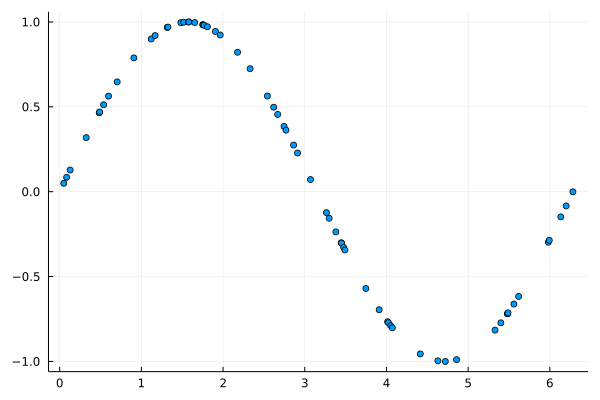
\includegraphics[width=0.8\textwidth]{images/nu_points.png}
    \caption{Non uniform sample points}
    \label{fig:nu_points}
\end{figure}

Using these samples, we can fit a simple piece-wise linear interpolation to sample uniform points as seem in Figure~\ref{fig:images-interp-png}.
\begin{figure}[htpb]
    \centering
    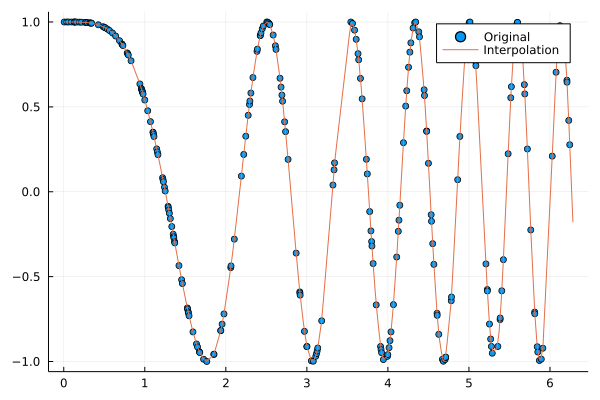
\includegraphics[width=0.8\textwidth]{images/interp.png}
    \caption{Piece-wise linear interpolant of non-uniform points}
    \label{fig:images-interp-png}
\end{figure}

In comparison, we can smooth the non-uniform points using the exponential of semicircle kernel as described in the previous section.
This convolution results in uniform samples as seen in Figure~\ref{fig:images-es-png}.
\begin{figure}[htpb]
    \centering
    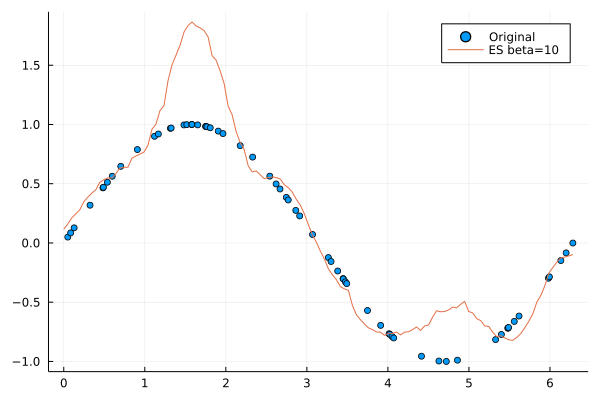
\includegraphics[width=0.8\textwidth]{images/es.png}
    \caption{Exponential of semicircle convolution of non-uniform sample points}
    \label{fig:images-es-png}
\end{figure}

Once resampled to uniform points, we can use the FFT to examine the Fourier spectrum of our samples.
\begin{figure}[htpb]
    \centering
    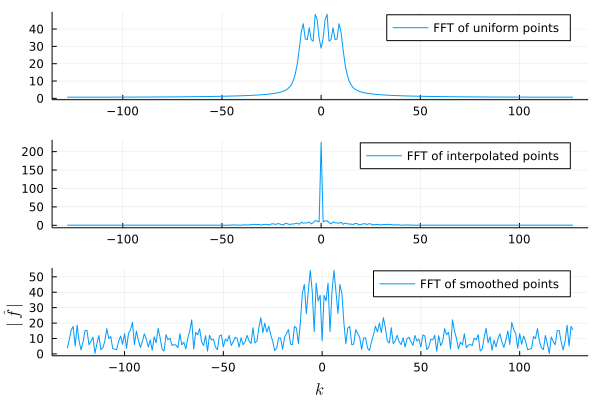
\includegraphics[width=0.8\textwidth]{images/fft_comparison.png}
    \caption{Comparison of spectra for uniform fft, interpolated fft, and smoothed nufft}
    \label{fig:images-fft-png}
\end{figure}

As expected, we can observe the reduction in accuracy using smoothing kernels as compared to the polynomial interpolation.
However, we can also quickly see the reduction in computational cost between the methods.
Figure~\ref{fig:images-speed-png} shows the speed of the approaches as a function of the number of non-uniform samples.
\begin{figure}[htpb]
    \centering
    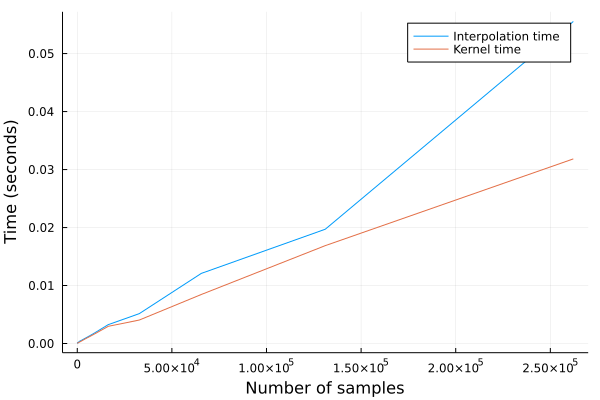
\includegraphics[width=0.8\textwidth]{images/speed.png}
    \caption{Comparison of method speed between interpolating and kernel methods}
    \label{fig:images-speed-png}
\end{figure}